% Template for Cogsci submission with R Markdown

% Stuff changed from original Markdown PLOS Template
\documentclass[10pt, letterpaper]{article}

\usepackage{cogsci}
\usepackage{pslatex}
\usepackage{float}
\usepackage{caption}

% amsmath package, useful for mathematical formulas
\usepackage{amsmath}

% amssymb package, useful for mathematical symbols
\usepackage{amssymb}

% hyperref package, useful for hyperlinks
\usepackage{hyperref}

% graphicx package, useful for including eps and pdf graphics
% include graphics with the command \includegraphics
\usepackage{graphicx}

% Sweave(-like)
\usepackage{fancyvrb}
\DefineVerbatimEnvironment{Sinput}{Verbatim}{fontshape=sl}
\DefineVerbatimEnvironment{Soutput}{Verbatim}{}
\DefineVerbatimEnvironment{Scode}{Verbatim}{fontshape=sl}
\newenvironment{Schunk}{}{}
\DefineVerbatimEnvironment{Code}{Verbatim}{}
\DefineVerbatimEnvironment{CodeInput}{Verbatim}{fontshape=sl}
\DefineVerbatimEnvironment{CodeOutput}{Verbatim}{}
\newenvironment{CodeChunk}{}{}

% cite package, to clean up citations in the main text. Do not remove.
\usepackage{cite}

\usepackage{color}

% Use doublespacing - comment out for single spacing
%\usepackage{setspace}
%\doublespacing


% % Text layout
% \topmargin 0.0cm
% \oddsidemargin 0.5cm
% \evensidemargin 0.5cm
% \textwidth 16cm
% \textheight 21cm

\title{Measuring lay theories of parenting and child development}


\author{{\large \bf Emily Hembacher} \\ \texttt{ehembach@stanford.edu} \\ Department of Psychology \\ Stanford University \And {\large \bf Michael C. Frank} \\ \texttt{mcfrank@stanford.edu} \\ Department of Psychology \\ Stanford University}

\begin{document}

\maketitle

\begin{abstract}
Child development research suggests that parenting practices play an
important role in shaping children's outcomes. For example, children
whose parents engage them in high-quality conversations and who are
given opportunities for free play are at an advantage for learning and
later academic outcomes. However, communicating the results of relevant
scientific findings to parents remains a challenge. One possible
moderator of uptake of parenting information is the implicit theories
parents hold with regard to child development and parenting. As a first
step in investigating this possibility, the present work establishes a
new measure of parenting attitudes, and examines whether scores on three
subscales, corresponding to lay theories about rules and respect,
affection and attachment, and early learning, differentially predict
uptake of a popular press article about children's early learning.
Scores on the early learning subscale, but not the rules and respect
subscale, predicted generalization from the article, providing first
evidence of the validity of this measure.

\textbf{Keywords:}
Parenting attitudes; implicit theories
\end{abstract}

Child development research is constantly generating information that can
be brought to bear on best-practices for parenting. For example,
research on children's learning has demonstrated that pedagogy can
improve learning in some contexts and limit it in others, suggesting
that allowing children to play freely and explore is critical for
learning (Bonawitz et al., 2011; Buchsbaum, Gopnik, Griffiths, \&
Shafto, 2011). Likewise, a great deal of research has demonstrated the
importance of engaging young children in elaborative conversations for
language development and future academic success (Hart \& Risley, 1995;
Hoff, 2003; Huttenlocher, Waterfall, Vasilyeva, Vevea, \& Hedges, 2010).
A fundamental challenge we face is how to communicate the results of
such scientific inquiry to a diverse public in a way that maximizes
uptake and improves people's daily and long-term decision making.

One critical parameter that may mediate parenting behavior is parents'
implicit lay theories about child development and parenting. Lay
theories reflect the core beliefs that people hold in different domains,
which may or may not be explicitly articulated, but organize the
processing of new information and decision-making (Dweck \& Leggett,
1988; Ong, Zaki, \& Goodman, 2015). For example, people with an entity
theory of personality tend to interpret people's behaviors as stemming
from fixed personality traits rather than situational factors such as
needs, goals, or emotional states (Dweck, Chiu, \& Hong, 1995).

There are two reasons to focus on parents' lay theories. First, parents'
lay theories might be an important explanatory factor for many of the
behaviors parents engage in with their child. For example, a parent who
believes that building a strong emotional bond with their baby is one of
the most important goals of parenting might have more physical contact
with their child than a parent who does not hold this theory. Secondly,
parents' lay theories may moderate the uptake of new information about
parenting. It is well-established that people more easily encode new
information that is consistent with an existing schema or mental model
they hold (Bransford \& Johnson, 1972). In addition, previous research
has found that interventions on public health beliefs are more
successful when they take into account people's existing belief
structures in the domain (V. Kumar et al., 2015).

There is some evidence supporting the notion that parents' behaviors are
mediated by implicit lay theories about child development, which vary by
SES and across cultures. For example, cross-cultural studies have found
profound differences in how parents interact with infants. Richman,
Miller, \& LeVine (1992) found that mothers in the Gusii community of
Kenya primarily engaged with their children to soothe them when upset,
but did not often speak to them with the goal of engaging or stimulating
them, as did Caucasian parents in the United States. The authors
attribute this to cultural conventions stemming from the belief that
there is no purpose in speaking to infants as they will not understand
what is being said (LeVine, 2004; Richman et al., 1992).

There are also important differences in how parents within western
cultures interact with their children. Numerous studies have identified
SES disparities in the amount that parents talk to their children, which
predicts children's language and academic outcomes (Hoff, 2003;
Huttenlocher, Vasilyeva, Cymerman, \& Levine, 2002). In an effort to
identify the source of this disparity, Rowe (2008) discovered that
parents' knowledge of child development (as indexed by their scores on
the Knowledge of Infant Development Inventory; KIDI) predicted their
child-directed language, with more knowledgeable parents speaking to
their children more even when controlling for the amount of speech
directed at another adult. Although this study examined parents'
knowledge, and not their lay theories \emph{per se}, it provides
evidence that people's domain knowledge has real consequences for their
interactions with their children.

\begin{table*}[t]
\centering
\begin{tabular}{p{1.25in}p{5.25in}}
  \hline
Subscale & Full item \\ 
  \hline
Rules/Respect & It is very important that children learn to respect adults, such as parents and teachers. \\ 
   & It is important for young children to learn to control their impulses (e.g., waiting when told to wait). \\ 
  & Children should be taught to be grateful to their parents. \\ 
  & Children should not be punished for breaking small rules.* \\ 
  & Parents should follow their childrens lead rather than imposing structure in the form of rules.* \\ 
  & Young children should be allowed to make their own decisions, such as what to eat for dinner.* \\ 
  \hline
  Affection/Attachment & Parents need to provide safe and loving environments for their children. \\ 
   & Holding and cradling babies is important for forming strong bonds between parent and child. \\ 
   & Children should be given comfort and understanding when they are scared or unhappy. \\ 
   & Parents do not need to talk to their child about his or her emotions.* \\ 
   & Children become spoiled if they receive too much attention from parents.* \\ 
   & Too much affection can make a child weak.* \\ 
   \hline
  Early Learning & Children can learn about things like good and bad behavior from a very early age. \\ 
   & Young children can teach themselves things by exploring and playing. \\ 
   & Babies repetitive behaviors (e.g., banging a cup on the table) are a way for them to explore cause and effect. \\ 
   & It is not helpful for adults to explain the reasons for rules to young children because they won't understand.* \\ 
   & Children don't need to learn about numbers and math until they go to school.* \\ 
   & Reading books to children is not helpful if they have not yet learned to speak.* \\ 
   \hline
   *Reverse coded
\end{tabular}
\caption{Parenting Attitudes Scale items.\label{tab:items}} 
\end{table*}

There are other examples of parenting beliefs on which parents differ.
For example, Lareau (2003)`s theory of ``concerted cultivation''
suggests that higher SES parents are more likely to view their child's
development as a project that requires a great deal of coordination in
the form of activities and learning experiences, while lower SES parents
are more likely to view their job as keeping their children safe from
harm, with the assumption that they will naturally thrive if given
independence. There have also been hundreds of studies based on Baumrind
(1971)'s framework that identifies parents as authoritative,
authoritarian, or permissive, based on their levels of responsiveness
and control in their interactions with their children. Thus, parents'
approaches to parenting appear to vary in predictable ways based on
their knowledge and perceptions about children's learning and
development.

Although these previous studies provide preliminary evidence that
parents' beliefs about parenting and child development affect their
parenting behaviors, no previous research has attempted to identify the
underlying theories that might organize their behavior and
decision-making. Previous research has generally relied on observation
of parent-child interactions or self-report of specific activities and
behaviors. To our knowledge there is not an existing measure of parents'
more general attitudes about parenting and child development, which
might drive behavior and predict the uptake of interventions.

To address this gap, the present work establishes a self-report scale
that captures adults' lay theories about child development and
parenting. We generated a questionnaire measuring the degree to which
parents endorse three potential lay theories: a ``rules and respect''
theory, an ``affection and attachment'' theory, and an ``early
learning'' theory. As an initial test of the external validity of the
questionnaire, we conducted an experiment to investigate whether
parents' scores on the theory subscales would differentially predict
their uptake of parenting information presented via a popular press
article about children's early learning from free play A. Gopnik (2011).
We found that higher scores on the ``early learning'' subscale, but not
the ``rules and respect'' subscale, predicted recall and generalization
from the target article (about free play) but not a control article that
was unrelated to child development. Thus, parents' lay theories about
parenting and child development as measured by our questionnaire may be
a meaningful factor in parents' behavior and information uptake.

\section{Scale Construction}\label{scale-construction}

In order to establish a new measure of parenting attitudes, we followed
a structured plan based on psychometric best practices (Clark \& Watson,
1995; Furr, 2011; Simms, 2008). We generated items corresponding to
three hypothesized latent theories about parenting: the Early Learning
theory corresponds to a view of children's early learning that is
consistent with contemporary child development research, and includes
the idea that young children can teach themselves by exploring and
playing. The Affection and Attachment theory captures the notion that
close parent-child relationships are important for development, and
includes the ideas that parents should talk to their children about
their emotions and that children are not spoiled by too much affection.
The Rules and Respect theory corresponds to the idea that parents'
primary role is to enforce rules and encourage behavior control. We
generated items based on a review of the literature on parenting
attitudes, and conducted psychometric analyses on iterative samples of
respondents collected on Amazon Mechanical Turk, both parents and
non-parents (seven in total).

\begin{CodeChunk}
\begin{figure*}

{\centering 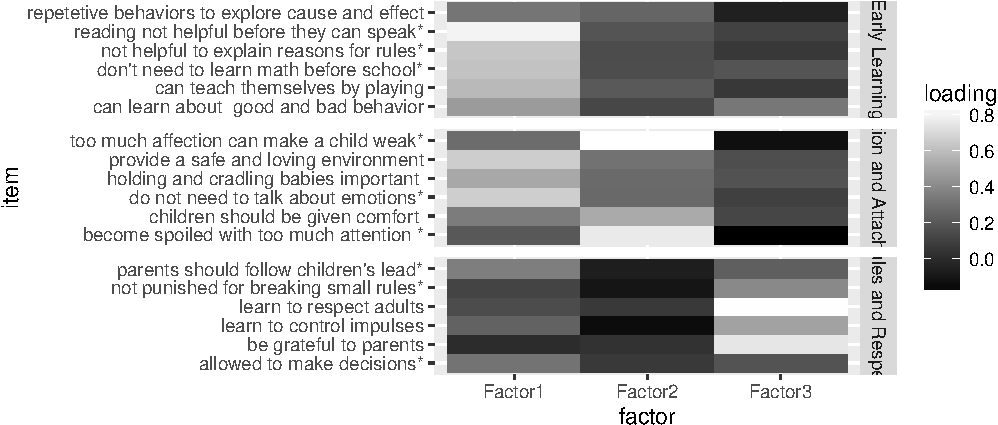
\includegraphics{figs/loadings-1} 

}

\caption[Factor loadings for subscale items]{Factor loadings for subscale items.}\label{fig:loadings}
\end{figure*}
\end{CodeChunk}

\subsection{Item construction}\label{item-construction}

In an initial phase of scale construction, we generated 42 statements
that described attitudes consistent with one of three potential implicit
theories about parenting: Active Learning (12 items; e.g., ``Children
can learn about things like good and bad behavior from an early age''),
Affection and Attachment (10 items; e.g., ``It's important for a baby to
have a strong bond with mom''), and Rules and Respect (20 items; e.g.,
``It is very important that children learn to respect adults, such as
parents and teachers''). These statements were generated based on a
literature review of parenting attitudes and behaviors. The Affection
and Attachment and Rules and Respect subscales are related theoretically
to the Authoritative and Authoritarian dimensions of Baumrind (1971)'s
parenting framework, as well as theories of attachment parenting (Jones,
Cassidy, \& Shaver, 2014), but aim to assess beliefs about parenting
rather than overt behaviors. The Early Learning subscale aimed to assess
the extent to which adults believe that it is important to help infants
and toddlers learn through play and conversation.

The initial 42-item scale was administered to 250 adults on Amazon's
Mechanical Turk. Participants used a 7-point Likert scale to report the
degree to which they agreed with each statement from 0 (Do not Agree) to
6 (Strongly Agree). Cronbach's alphas for the three subscales were .86
(Active Learning), .81 (Affection and Attachment), and .74 (Rules and
Respect). We then conducted Exploratory Factor Analysis (EFA) to assess
the dimensionality of the scale. Based on a parallel analysis (Horn,
1965), we retained 5 factors in this initial model. We subsequently
dropped any items that had factor loadings less than .40 on the relevant
factor, as well as any items that had factor loadings greater than .40
onto another factor. Items were also dropped if analyses revealed that
Cronbach's alpha would be increased by dropping the item. Additional
items were dropped such that there were 6 items in each subscale. Some
items were re-worded such that half of the items in each subscale were
negatively worded to avoid response sets (Simms, 2008).

\subsection{Revised questionnaire
norming}\label{revised-questionnaire-norming}

The revised questionnaire was administered to a second group of 250
adults on Amazon's Mechanical Turk. Table \ref{tab:items} gives the full
list of items. For this sample, Cronbach's alphas were .76 (Active
Learning), .75 (Affection and Attachment), and .69 (Rules and Respect).
Because analysis of the previous sample identified 5 factors instead of
the hypothesized 3, we again conducted EFA. This time, the parallel
analysis identified 3 factors as predicted. We next examined the
loadings of individual items onto the three factors (Figure
\ref{fig:loadings}). Items loaded onto the three factors roughly
consistent with our a priori subscales, although some items from the
Affection and Attachment subscale loaded onto both the Affection and
Attachment and Active Learning factors. Given the loadings of Early
Learning and Affection and Attachment items onto a single factor, it is
possible that participants responses on these items were driven by a
more general hands-on attitude towards parenting, similar to Lareau's
(2003) Concerted Cultivation theory. Interestingly, when we conducted an
exploratory analysis of factor loadings by gender, we found that female
gender loaded highly positively onto the Affection and Attachment factor
that did not include Early Learning items (.44), while the opposite was
true for male gender (-.20). Thus, it is possible that these items
reflect a theory related to Affection and Attachment that is seperable
from the hands-on approach and differentiated by gender.

\begin{table*}[!h]
\centering
\begin{tabular}{p{1.25in}p{5.25in}}
  \hline
Uptake category \\ 
  \hline
Control recall 
& According to Article 2, what do the groups known for having many words for smells have in common? \\ 
  & A) They train their children to be able to tell the difference between smells.\\ 
  & B) They are hunter-gatherers.*\\ 
  & C) They have unusually good hearing and vision.\\ 
\hline
Target recall
  & According to Article 1, children were more likely to find new and better ways to make a toy work when the experimenter:\\ 
  & A) Pretended to be clueless about how the toy worked when playing with it.*\\ 
  & B) Pretended to be an expert about the toy when playing with it.\\ 
  & C) Pretended not to care about the toy.\\ 
  \hline
  Target generalization 
  & Based on Article 1, preschool directors should plan to have:\\ 
  & A) More structured time in which children are taught lessons and skills.\\ 
  & B) More time spent memorizing things that will be helpful later, such as the ABCs.\\
  & C) More time for children to play outside and with toys.*\\
   \hline
*Correct answer   
\end{tabular}
\caption{Examples of uptake questions.\label{tab:uptake}} 
\end{table*}

As one test of the external validity of the subscales, we fit linear
mixed-effects models predicting subscale scores based on gender and
parenthood status (i.e., whether or not the participant reported having
children) with participants as random effects. The model including
gender revealed that females had higher scores on Early Learning, β =
0.41, SE = .19, and Affection and Attachment β = 0.34, SE = .23, whereas
gender had no effect on Rules and Respect scores. The model including
parenthood status revealed that parents had higher scores on the
Affection and Attachment subscale compared to non-parents, β = 0.35, SE
= 13, whereas parenthood status had no effect on Early Learning or Rules
and Respect scores. Although it is not possible to determine the source
of these differences, they provide some intuitive support for the notion
that subscale scores tap meaningful constructs that vary across groups.

\subsection{Initial Validity Evidence}\label{initial-validity-evidence}

\section{Experiment 1}\label{experiment-1}

We next conducted an experiment to test whether scores on the three
subscales would predict people's uptake of new information, as an
initial test of the external validity of the scales. For this purpose,
we had participants read two popular press articles: an article arguing
that free play is beneficial to children's learning (A. Gopnik, 2011),
and a control article about the language of smell (Yong, 2015). We
operationalized uptake as accurate recall and generalization of the
central message of the target article, and recall of the control
article. We predicted that if people's subscale scores reflect coherent
lay theories, they should differentially moderate uptake of the two
articles. Specifically, we predicted that scores on the Early Learning
subscale would be positively related to recall and generalization of the
target article, but not recall of the control article. We predicted that
scores on the Rules and Respect subscale would not predict uptake of
either article. We excluded scores on the Affection and Attachment
subscale from our analyses, since they are not orthogonal to scores on
the Early Learning subscale.

\subsection{Methods}\label{methods}

\subsubsection{Participants}\label{participants}

Participants were 250 adults recruited from Amazon Mechanical Turk. Of
these participants, 123 reported having children, 122 reported having no
children, and 5 did not respond.

\subsubsection{Procedure}\label{procedure}

Participants first completed the 18-item parenting questionnaire
described above. Participants were then instructed to read two popular
press articles at their own pace. They first read a target article about
children's early learning (``Why Preschool Shouldn't Be Like School,''
Alison Gopnik, Slate, 2011), and then read a control article about the
language of smell (``Why Do Most Languages Have So Few Words For
Smells?'', Ed Yong, The Atlantic, 2015). After reading both articles,
they first answered five 3-alternative forced-choice recall questions
about the control article, and then answered five 3AFC generalization
and five 3AFC recall questions about the target article. The recall
questions assessed participants' memory for specific details of the
text, and the generalization questions assessed participants' ability to
generalize from the meaning of the text to new situations (Table
\ref{tab:uptake}). The alternative choices for recall and generalization
questions were designed to reflect reasonable options that were
nonetheless inconsistent with the articles.

\subsection{Results and discussion}\label{results-and-discussion}

We excluded 48 participants who spent less than 30 seconds reading one
or both of the articles, based on the assumption that they had not had
time to read the whole article. Mean accuracy for the remaining sample
was 0.6712871 (SD = 0.2361956) for control recall, 0.8346535 (SD =
0.193905) for target recall, and 0.8742574 (SD = 0.2181576) for target
generalization.

\begin{CodeChunk}
\begin{figure*}[h]

{\centering 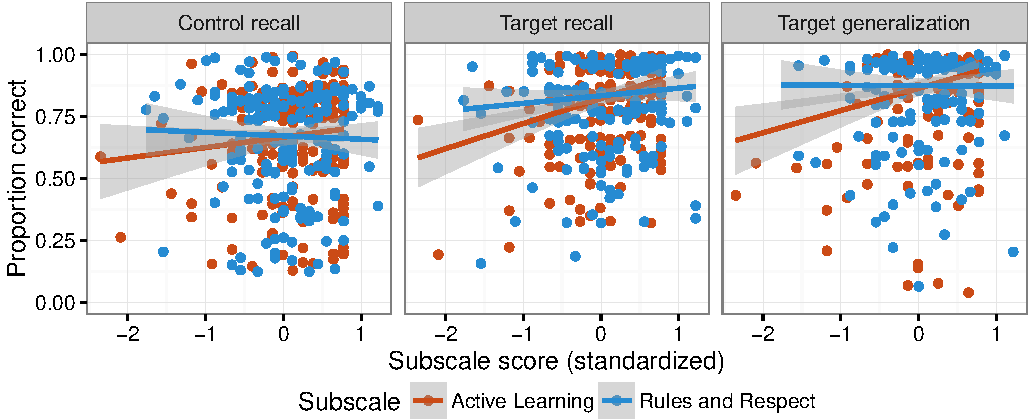
\includegraphics{figs/relation-1} 

}

\caption[Relationship between subscale scores and uptake of articles]{Relationship between subscale scores and uptake of articles.}\label{fig:relation}
\end{figure*}
\end{CodeChunk}

Figure \ref{fig:relation} shows proportion correct on each of the three
trial types, plotted by standardized subscale scores. Regression lines
show the relationship between subscale scores and proportion correct.
Qualitatively, there was not strong evidence of a relationship between
Rules and Respect scores and performance (though Target recall showed
some trend). In contrast, we observed a stronger relationship between
performance and Active Learning scores, most especially for Target
generalization trials.

To quantify these trends, we fit a generalized linear mixed-effects
model with standardized Early Learning and Rules and Respect subscale
scores, as well as interaction terms for the subscale scores by question
type (i.e., control recall vs.~target recall vs.~target generalization)
as fixed effects, and participants and questions as random
effects.\footnote{This random effects specification was the maximal
  convergent random effect structure.} Coefficient estimates are shown
in Table \ref{tab:lmer}. Early Learning scores interacted positively
with target recall and target generalization to predict correct
performance, whereas Rules and Respect scores interacted positively with
target recall but not target generalization, and coefficient magnitudes
were relatively lower. Thus, Active Learning scores differentially
predicted generalization from the target passage.\footnote{These results
  held when Affection/Attachment items were included in the analysis as
  well. Affection/Attachment scores also moderated generalization,
  though not as strongly as Early Learning scores.}

\begin{table}[t]
\centering
\begin{tabular}{lrrrr}
  \hline
Predictor & Estimate & Std. Error & z value & $p$ \\ 
  \hline
  Cntl recall & 1.11 & 0.37 & 2.98 & 0.00 \\ 
  Targ gen & 1.57 & 0.49 & 3.19 & 0.00 \\ 
  Targ recall & 1.28 & 0.49 & 2.59 & 0.01 \\ 
  Rules/Respect & -0.10 & 0.21 & -0.48 & 0.63 \\ 
  Active Learning & 0.27 & 0.22 & 1.22 & 0.22 \\ 
  Targ gen $\times$ R/R & -0.06 & 0.06 & -0.94 & 0.35 \\ 
  Targ recall $\times$ R/R& 0.32 & 0.06 & 5.62 & 0.00 \\ 
  Targ gen $\times$ AL & 0.62 & 0.06 & 10.86 & 0.00 \\ 
  Targ recall $\times$ AL & 0.49 & 0.05 & 8.97 & 0.00 \\ 
   \hline
\end{tabular}
\caption{Fixed-effect coefficients for linear mixed effects model predicting task performance in Experiment 1. AL = Active Learning; RR = Rules and Respect.\label{tab:lmer}} 
\end{table}

\section{General Discussion}\label{general-discussion}

Understanding the sources of parents' behaviors and decisions with
regard to their parenting is a critical step in improving children's
welfare. There is a large literature outlining the activities and
environments that can make a difference in children's development,
including their language (Hart \& Risley, 1995), executive functioning
(Barker et al., 2014), and conceptual learning (Bonawitz et al., 2011).
Relevant research findings can sometimes be nuanced and unintuitive for
those outside of academia, however. Thus, an important challenge is
understanding the lay beliefs parents may have about parenting, and how
they relate to parenting best-practices as identified by developmental
science. Interventions that aim to deliver new information may be more
likely to succeed if they take into account the existing lay beliefs
that parents hold about child development (V. Kumar et al., 2015).

In the present work, we established a new scale to measure people's
attitudes about parenting and child development in three categories:
Rules and Respect, Affection and Attachment, and Early learning. These
subscales are meant to capture meaningful differences in how people view
child development and the relative importance of different parenting
behaviors. We subjected our new scale to psychometric testing, and found
acceptably high correlations among subscale items, as well as the
predicted factor structure across subscales. In addition, subscale
scores meaningfully predicted uptake of new information about parenting.
Specifically, participants with high scores on the Early Learning
subscale were more likely to generalize the message of the target
article about children's learning to new scenarios, whereas high scores
on the Rules and Respect subscale did not predict generalization of the
article.

One possibility that deserves consideration is that participants who
scored higher on the Active Learning subscale would have been more
likely to respond correctly to the target generalization and recall
questions even without having read the article. It is very possible that
adults who believe that children's early learning is a priority, and who
believe young children are capable of learning a lot, are more likely to
already possess the knowledge presented in the target article, or might
intuitively answer the questions based on their implicit theories of
children's learning. Although this would mean their advantage on the
target generalization items might not stem from better generalization of
concepts consistent with their implicit theories, it would still provide
validation that subscale scores are predictive of how parents reason
about children's learning.

In sum, this work provides initial evidence that meaningful differences
in adults' attitudes about child development and parenting can be
assessed by our new scale. This initial evidence for the reliability and
validity of our parenting measure must be supplemented with further
evidence in both areas across a broader range of participants. In
addition, future work should target predictive validity by determining
whether subscale scores differentially predict parents observable
behaviors with their children, such as the quality of conversations they
engage their child in, which would provide additional support for our
scale.

Implicit theories are a powerful driver of human behavior. Often, the
interaction between interventions and their subjects' underlying beliefs
can produce powerful, non-linear results. Thus, given both the
variability in attitudes towards parenting across cultures and the
importance of improving parenting outcomes, it behooves us to understand
implicit theories of parenting. The current work takes a first step in
this direction.

\section{Acknowledgements}\label{acknowledgements}

This work supported by a gift from Kinedu, Inc. Thanks to members of the
Language and Cognition Lab at Stanford for helpful discussion.

\section{References}\label{references}

\small

Barker, J. E., Semenov, A. D., Michaelson, L., Provan, L. S., Snyder, H.
R., \& Munakata, Y. (2014). Less-structured time in children's daily
lives predicts self-directed executive functioning. \emph{Frontiers in
Psychology}, \emph{5}, 323.

Baumrind, D. (1971). Current patterns of parental authority.
\emph{Developmental Psychology}, \emph{4}(1p2), 1--103.

Bonawitz, E., Shafto, P., Gweon, H., Goodman, N. D., Spelke, E., \&
Schulz, L. (2011). The double-edged sword of pedagogy: Instruction
limits spontaneous exploration and discovery. \emph{Cognition},
\emph{120}(3), 322--330.

Bransford, J. D., \& Johnson, M. K. (1972). Contextual prerequisites for
understanding: Some investigations of comprehension and recall.
\emph{Journal of Verbal Learning and Verbal Behavior}, \emph{11}(6),
717--726.

Buchsbaum, D., Gopnik, A., Griffiths, T. L., \& Shafto, P. (2011).
Childrens imitation of causal action sequences is influenced by
statistical and pedagogical evidence. \emph{Cognition}, \emph{120}(3),
331--340.

Clark, L. A., \& Watson, D. (1995). Constructing validity: Basic issues
in objective scale development. \emph{Psychological Assessment},
\emph{7}(3), 309--319.

Dweck, C. S., \& Leggett, E. L. (1988). A social-cognitive approach to
motivation and personality. \emph{Psychological Review}, \emph{95}(2),
256--273.

Dweck, C. S., Chiu, C.-y., \& Hong, Y.-y. (1995). Implicit Theories:
Elaboration and Extension of the Model. \emph{Psychological Inquiry},
\emph{6}(4), 322--333.

Furr, M. (2011). \emph{Scale Construction and Psychometrics for Social
and Personality Psychology}. SAGE Publications Ltd.

Gopnik, A. (2011). Why preschool shouldn't be like school. \emph{Slate
Magazine}.

Hart, B., \& Risley, T. R. (1995). \emph{Meaningful Differences in the
Everyday Experience of Young American Children}. Paul H Brookes
Publishing Company.

Hoff, E. (2003). The Specificity of Environmental Influence:
Socioeconomic Status Affects Early Vocabulary Development Via Maternal
Speech. \emph{Child Development}, \emph{74}(5), 1368--1378.

Horn, J. L. (1965). A rationale and test for the number of factors in
factor analysis. \emph{Psychometrika}, \emph{30}(2), 179--185.

Huttenlocher, J., Vasilyeva, M., Cymerman, E., \& Levine, S. (2002).
Language input and child syntax. \emph{Cognitive Psychology},
\emph{45}(3), 337--374.

Huttenlocher, J., Waterfall, H., Vasilyeva, M., Vevea, J., \& Hedges, L.
V. (2010). Sources of variability in childrens language growth.
\emph{Cognitive Psychology}, \emph{61}(4), 343--365.

Jones, J. D., Cassidy, J., \& Shaver, P. R. (2014). Parents
Self-Reported Attachment Styles A Review of Links with Parenting
Behaviors, Emotions, and Cognitions. \emph{Personality and Social
Psychology Review}, \emph{19}(1), 1088868314541858--76.

Kumar, V., Kumar, A., Ghosh, A. K., Samphel, R., Yadav, R., Yeung, D.,
\& Darmstadt, G. L. (2015). Enculturating science: Community-centric
design of behavior change interactions for accelerating health impact.
\emph{Seminars in Perinatology}, \emph{39}(5), 393--415.

Lareau, A. (2003). \emph{Unequal Childhoods}. Univ of California Press.

LeVine, R. A. (2004). \emph{Challenging Expert Knowledge: Findings from
an African Study of Infant Care and Development.} Praeger
Publishers/Greenwood Publishing Group.

Ong, D. C., Zaki, J., \& Goodman, N. D. (2015). Affective cognition:
Exploring lay theories of emotion. \emph{Cognition}, \emph{143},
141--162.

Richman, A. L., Miller, P. M., \& LeVine, R. A. (1992). Cultural and
educational variations in maternal responsiveness. \emph{Developmental
Psychology}, \emph{28}(4), 614--621.

Rowe, M. L. (2008). Child-directed speech: relation to socioeconomic
status, knowledge of child development and child vocabulary skill.
\emph{Journal of Child Language}, \emph{35}(01), 185--205.

Simms, L. J. (2008). Classical and Modern Methods of Psychological Scale
Construction. \emph{Social and Personality Psychology Compass},
\emph{2}(1), 414--433.

Yong, E. (2015). Why do most languages have so few words for smells?
\emph{The Atlantic}.

\end{document}
